\documentclass[journal]{IEEEtran}
\usepackage{cite}
\usepackage{amsmath,amssymb,amsfonts}
\usepackage{graphicx}
\usepackage{xcolor}
\usepackage{url}
\usepackage[caption=false,font=footnotesize]{subfig}
\usepackage[ruled,vlined,linesnumbered]{algorithm2e}
\newtheorem{proposition}{Proposition}
\newtheorem{lemma}{Lemma}

\begin{document}

\title{Accuracy-Aware ISCC Optimization for Aerial Edge Inference in SI-TNTNs}

\author{Thien~Hieu~Hoang, Tri~Nhu~Do, and Georges~Kaddoum%
\thanks{T.~H.~Hoang and G.~Kaddoum are with the Department of Electrical Engineering, \'{E}TS, Montr\'{e}al, Qu\'{e}bec, Canada (e-mail: \mbox{thien-hieu.hoang.1@ens.etsmtl.ca}; \mbox{Georges.Kaddoum@etsmtl.ca}). T.~N.~Do is with the Department of Electrical Engineering, Polytechnique Montr\'{e}al, Montr\'{e}al, Qu\'{e}bec, Canada (e-mail: \mbox{tri-nhu.do@polymtl.ca}).}}
\maketitle

\begin{abstract}
We study integrated sensing, communication, and computation (ISCC) for uplink--downlink coexistence edge inference over stochastic integrated terrestrial and non-terrestrial networks (SI-TNTNs). Ground user equipments sense their environment, compress the raw observation into a feature payload, and partially offload the resulting inference task to hovering unmanned aerial vehicles hosting inference servers in 3D space, while jammers impair both links. Node locations follow homogeneous Poisson point processes. Using matched-filter successive interference cancellation on the uplink and zero-forcing beamforming on the downlink, we formulate a mixed-integer nonlinear program trading off delay, energy, downlink rate, and inference accuracy. Both sensing-induced variables admit closed forms (the three-point delay--energy offloading split and the utility-optimal feature-retention ratio), so the ISCC extension leaves the search complexity of the whale/particle-swarm solver unchanged.
\end{abstract}

\begin{IEEEkeywords}
ISCC, UAV edge inference, SI-TNTN, partial offloading, inference accuracy, resource allocation, whale optimization.
\end{IEEEkeywords}

\section{Introduction}
Sixth-generation networks are expected to deliver sensing, communication, and computation as one service. Integrated sensing, communication, and computation (ISCC) changes the figure of merit accordingly: what matters is the accuracy of the inference the sensed data supports, not the rate at which its bits arrive. Stochastic integrated terrestrial and non-terrestrial networks (SI-TNTNs) \cite{meftah2026sitntn} host such services naturally, unmanned aerial vehicles (UAVs) carrying servers beyond fixed terrestrial cells at positions neither planned nor static, so performance must hold in distribution over deployments.

Edge inference is the workload: a device senses, extracts features, and forwards part of them to a UAV-hosted server. How aggressively the observation is compressed before transmission is one knob fixing accuracy, airtime, and server cycles at once, so the three functions share a single budget. Coexisting uplink (UL) and downlink (DL) complicates it: half-duplex UAVs reusing sub-channels leak power between offloading UL and broadcasting DL, successive interference cancellation leaves residual intra-cell interference and decoding-margin constraints, zero-forcing (regularized when overloaded) nulls intra-cell DL interference, and jammers corrupt both directions. All enter the achievable rates, hence the delay and energy against which compression is priced.

The resulting mixed-integer nonlinear program couples association, powers, server frequencies, and the sensing-induced variables through interference, and is NP-hard \cite{Hoang_TCOM_2024}, so swarm heuristics \cite{book_SI2010,genetic_optim} are the usual recourse. Prior work is fragmented with respect to this setting. ISCC supplies the accuracy objective, through discriminant-gain task-oriented compression \cite{wen2024iscc} and, more recently, energy-efficient split edge inference \cite{yao2025edgeinf}, but on single-cell terrestrial topologies with deterministic geometry and no jamming \cite{wen2025survey}. Non-terrestrial designs address integrated communication and computation under uncertainty \cite{tang2025ntn}, and sensing-offloading scheduling has been studied for multi-UAV edge inference \cite{du2026uavinf}, yet both assume a single link direction and benign spectra. None combines stochastic aerial geometry, UL--DL coexistence under jamming, and an inference-accuracy objective.

This letter recasts stochastic UL--DL edge inference on a SI-TNTN as an ISCC problem, contributing: (i) a planar-HPPP UAV edge-inference model with independent altitudes, jamming-aware MF-SIC and ZFBF, each UL UE sensing, compressing features at a tunable retention ratio, and partially offloading; (ii) an MINLP over delay, energy, DL rate, and accuracy; (iii) closed forms for both sensing-induced variables and a clipped water-filling compute rule, so ISCC adds no search cost; (iv) a hybrid WOA/IWOA/PSO--BWOA solver benchmarked against exhaustive search.

\section{System and Signal Models}
\label{sec:model}
Consider a square area with $M$ hovering UAVs (each with $L$ antennas and an onboard inference server), ground UEs, and ground jammers (Fig.~\ref{fig:sys}). UAVs are half-duplex, $M=M^{\tt ul}+M^{\tt dl}$. Bandwidth $B$ is reused over $K$ sub-channels of width $B_k=B/K$. Horizontal locations of UAVs, UEs, and jammers are independent 2D HPPPs $\Phi_0$, $\Phi_{\mathrm{UE}}$, $\Phi_{\mathrm{Q}}$ of intensities $\lambda_0$, $\lambda_{\mathrm{UE}}$, $\lambda_{\mathrm{Q}}$. Ground nodes sit on $z=z_{\min}$; UAV altitudes are drawn independently and uniformly from $[z_{\mathrm{uav}}^{\min},z_{\mathrm{uav}}^{\max}]$. UAV $m$, UE $n$, and jammer $q$ thus sit at $\vec{\ell}_m,\vec{\ell}_n,\vec{\ell}_q\in\mathbb{R}^3$. 
{\color{blue}Nearest-UAV association assigns each UE $n$ to UAV $m_n=\arg\min_m \Vert\vec{\ell}_m-\vec{\ell}_n\Vert_2$},
inducing Voronoi-like cells; 
the binary $\vec{A}^{\tt ul}$ then assigns a sub-channel, or local execution, inside the serving cell.

\begin{figure}[!t]
\centering
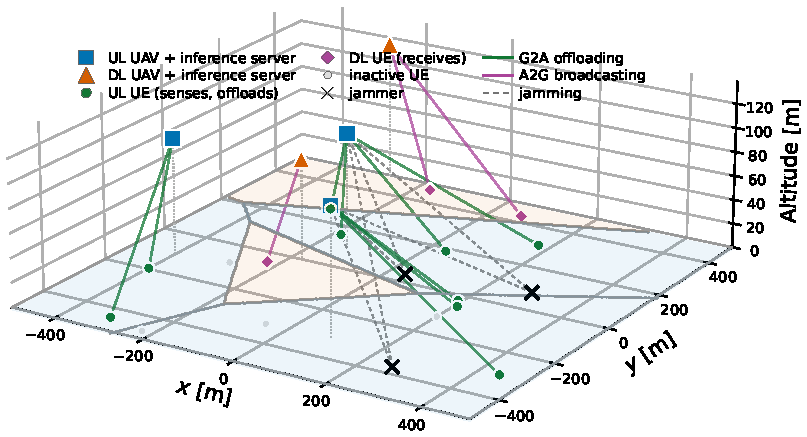
\includegraphics[width=\linewidth]{figures/topology3d_wGround.pdf}
\caption{One HPPP realisation of the SI-TNTN drawn by the simulator: UAVs hover at their sampled altitudes over ground UEs and jammers, with G2A offloading, A2G broadcasting, and jamming on both directions.}
\label{fig:sys}
\end{figure}

Each slot splits into an orthogonal sensing sub-slot, in which UL UEs acquire and compress their observations, and a communication sub-slot carrying UL offloading and DL broadcasting. Sensing thus contends for time and energy but not spectrum, leaving Secs.~\ref{sec:ul}--\ref{sec:dl} unaffected by the sensing waveform.

UL/DL UAV roles are an independent Bernoulli split with $\lambda_0^{\tt ul}=\lambda_0^{\tt dl}$.

For $\psi\in\{\tt G2A,A2G\}$,
$\vec{h}_{\mathrm{AB}}=\sqrt{\beta_{\mathrm{AB}}^{\psi}}\,\vec{g}_{\mathrm{AB}}\in\mathbb{C}^{L\times 1}$,
where $\beta_{\mathrm{AB}}^{\psi}=10^{-\mathrm{PL}^{\psi}_{\mathrm{AB}}/10}\,\zeta_{\mathrm{AB}}$ is the linear large-scale gain, $\mathrm{PL}^{\psi}$ is path loss in dB, $\zeta_{\mathrm{AB}}$ is inverse-Gamma shadowing, and $\vec{g}_{\mathrm{AB}}$ is Nakagami-$m$ fading with i.i.d.\ uniform phases. G2A path loss is $\mathrm{PL}^{\tt G2A}=10\alpha\log_{10}(d/d_0)+\mathrm{PL}_0$; A2G is $\mathrm{PL}^{\tt A2G}=\mathrm{FSPL}(d)+\eta_0$ with $\mathrm{FSPL}(d)=20\log_{10}(d)+20\log_{10}(f_c)-27.55$ for distance $d$ in metres and carrier $f_c$ in MHz, and excess loss $\eta_0$. Denote $\vec{h}_{n,k,m}$ the UE--UAV channel on sub-channel $k$.

\subsection{Sensing, Feature Extraction, and Accuracy}
\label{sec:sense}
Each UL UE $n\in\mathcal{N}^{\tt ul}$ illuminates its field of view for $\mathsf{T}_n^{\tt sen}$ at power $p_n^{\tt sen}$, at cost $\mathsf{E}_n^{\tt sen}=p_n^{\tt sen}\mathsf{T}_n^{\tt sen}$, and collects a raw observation of $D_n^{\tt raw}$ bits at sensing SNR $\gamma_n^{\tt sen}$. The sensing configuration $(\mathsf{T}_n^{\tt sen},p_n^{\tt sen})$ is part of the task descriptor; joint sensing-power control is left to future work. The UE then extracts features at $\varpi_n$ cycles/bit, costing $\mathsf{T}_n^{\tt ext}=\varpi_n D_n^{\tt raw}/F_n^{\tt loc}$ and $\mathsf{E}_n^{\tt ext}=\kappa_n\varpi_n D_n^{\tt raw}(F_n^{\tt loc})^2$ with switched-capacitance coefficient $\kappa_n$, and retains a fraction $\chi_n\in(0,1]$ of the extracted features. The surviving inference task is
\begin{equation}
I_n(\chi_n)=\{\chi_n D_n^{\tt raw},\,\chi_n C_n^{\tt raw},\,\gamma_n^{\tt sen}\},
\label{eq:task}
\end{equation}
i.e.\ retention scales payload and workload alike. Following the discriminant-gain view of task-oriented compression, in which classification accuracy grows with, and saturates in, the discriminant information carried by the retained features, we adopt the saturating surrogate
\begin{equation}
\Lambda_n(\chi_n)=1-e^{-\vartheta_n\chi_n \Gamma_n},
\qquad
\Gamma_n\triangleq\log_2(1+\gamma_n^{\tt sen}),
\label{eq:acc}
\end{equation}
with task sensitivity $\vartheta_n>0$, so that accuracy is increasing and concave in the retained feature information $\chi_n\Gamma_n$ and bounded by one. Thus $\chi_n$ is the single ISCC knob: raising it improves accuracy but inflates airtime, transmit energy, and server cycles simultaneously. Imposing $\Lambda_n\ge\Lambda^{\tt th}$ gives the retention floor
\begin{equation}
\chi_n^{\tt min}=-\ln(1-\Lambda^{\tt th})/(\vartheta_n \Gamma_n),
\label{eq:chimin}
\end{equation}
and UE $n$ is admissible only if $\chi_n^{\tt min}\le 1$, i.e.\ only if its sensing quality satisfies $\vartheta_n \Gamma_n\ge-\ln(1-\Lambda^{\tt th})$. When $\chi_n^{\tt min}>1$ the accuracy constraint is infeasible at any $\chi_n\le1$; such UEs leave the constraint set, execute locally, and are assigned zero utility.

\subsection{UL Partial Offloading and MF-SIC}
\label{sec:ul}
UE $n$ splits its task: a fraction $\rho_n\in[0,1]$ is offloaded and $1-\rho_n$ is executed locally at $F_n^{\tt loc}$. It has association $a_{n,k}^{\tt ul}\in\{0,1\}$ with $\sum_k a_{n,k}^{\tt ul}\le 1$, and power $p_n\in[0,p_n^{\tt max}]$. The all-local, full-retention reference costs are
\begin{align}
\mathsf{T}_n^{\tt ref}&=\mathsf{T}_n^{\tt sen}+\mathsf{T}_n^{\tt ext}+C_n^{\tt raw}/F_n^{\tt loc},
\label{eq:ref}\\
\mathsf{E}_n^{\tt ref}&=\mathsf{E}_n^{\tt sen}+\mathsf{E}_n^{\tt ext}+\kappa_n C_n^{\tt raw}(F_n^{\tt loc})^2 .
\nonumber
\end{align}
{\color{blue}For UE $i$, sub-channel $k$, UAV $m$, denote $\mathsf{g}_i\triangleq\Vert\vec{h}_{i,k,m}\Vert^2$, $c_{n,i}\triangleq|\vec{h}_{n,k,m}^{\sf H}\vec{h}_{i,k,m}|^2$, 
$\mathcal{N}_m^{\tt ul}=\{n:m_n=m\}$,
$\mathcal{N}_k^{\tt sub}=\{i:a_{i,k}^{\tt ul}=1\}$, and weaker intra-cell co-channel UEs $\mathcal{W}_{n,k,m}=\{i\in(\mathcal{N}_m^{\tt ul}\cap\mathcal{N}_k^{\tt sub})\setminus\{n\}:\mathsf{g}_i\le\mathsf{g}_n\}$.}
The received vector at UL UAV $m$ on sub-channel $k$ is
\begin{equation}
\begin{aligned}
\textstyle\vec{y}_{k,m}&=\textstyle\sum_{i\in\mathcal{N}_k^{\tt sub}}\vec{h}_{i,k,m}\sqrt{p_i}s_i+\sum_{m'\in\mathcal{M}_k^{\tt sub}}\vec{G}_{m',k,m}\vec{P}_{m',k}^{\tt UAV}\\
&\textstyle+\sum_{q\in\mathcal{Q}}a_{q,k}\vec{h}_{q,k,m}\sqrt{p_q}s_q+\vec{z}_{k,m},
\end{aligned}
\label{eq:ul_y}
\end{equation}
{\color{blue}with $\mathcal{M}_k^{\tt sub}$ the set of DL UAVs using sub-channel $k$ with transmit matrices $\vec{P}_{m',k}^{\tt UAV}$}, the UAV-to-UAV channel $\vec{G}_{m',k,m}\in\mathbb{C}^{L\times L}$, jammer activity $a_{q,k}\sim\mathrm{Bernoulli}(q_k)$ ($q_k$ is a probability, distinct from the DL powers $q_{m',n'}$), and $\vec{z}_{k,m}\sim\mathcal{CN}(\vec{0},N_0\vec{I}_L)$. MF-SIC uses $\vec{v}_{m,n}=\vec{h}_{n,k,m}$ and cancels stronger users first. The Signal-to-Interference-plus-Jamming-and-Noise Ratio (SIJNR) is
\begin{equation}
\gamma_{n,k,m}
=\frac{\mathsf{g}_n^2\, p_n}
{\mathcal{I}_{n,k,m}^{\tt w}\!+\mathcal{I}_{n,k,m}^{\tt o}\!+\mathcal{J}_{n,k,m}
\!+\mathsf{g}_n(\Xi_{k,m}/L+B_kN_0)},
\label{eq:ul_sijnr}
\end{equation}
where $\mathcal{I}_{n,k,m}^{\tt w}=\sum_{i\in\mathcal{W}_{n,k,m}}c_{n,i} p_i$ is residual intra-cell interference after SIC,
$\mathcal{I}_{n,k,m}^{\tt o}=\sum_{i\in\mathcal{N}_k^{\tt sub}\setminus(\mathcal{N}_m^{\tt ul}\cup\{n\})}c_{n,i} p_i$ is inter-cell UL interference,
$\Xi_{k,m}=\sum_{m'\in\mathcal{M}_k^{\tt sub}}\Vert\vec{G}_{m',k,m}\vec{P}_{m',k}^{\tt UAV}\Vert^2$, and
$\mathcal{J}_{n,k,m}=\sum_{q\in\mathcal{Q}}a_{q,k}c_{n,q} p_q$ is jamming, $\mathcal{Q}$ being the jammer set. 
Because the MF combiner is unnormalized, the projected noise is $\mathsf{g}_nB_kN_0$ and the isotropic DL leakage is $\mathsf{g}_n\Xi_{k,m}/L$, so both scale with $\mathsf{g}_n$ as the numerator does.
Reliable SIC requires a decoding margin $\epsilon_m^{\tt th}\ge1$,
\begin{equation}
\textstyle p_n\mathsf{g}_n\big/\sum_{i\in\mathcal{W}_{n,k,m}}p_i\mathsf{g}_i\ge\epsilon_m^{\tt th}.
\label{eq:sic}
\end{equation}
{\color{blue}If $\mathcal{W}_{n,k,m}=\emptyset$ (the cell-tail, decoded last), the constraint is vacuous.}
The transmission rate is $R_{n,k,m}=B_k\log_2(1+\gamma_{n,k,m})$, and $a_n^{\tt ul}=\sum_k a_{n,k}^{\tt ul}$ with $\rho_n\le a_n^{\tt ul}$ so that a UE without a sub-channel computes locally. The local branch and the offload branch run in parallel, so with $R_n\triangleq\sum_{m,k}a_{n,k}^{\tt ul}R_{n,k,m}$ and ignoring result-feedback payload,
\begin{align}
\mathsf{T}_n&=\mathsf{T}_n^{\tt sen}+\mathsf{T}_n^{\tt ext}+\chi_n\Delta_n,
\quad
\Delta_n=\max\{\Delta_n^{\tt loc},\Delta_n^{\tt ofl}\},
\label{eq:Tn}\\
\Delta_n^{\tt loc}&=\frac{(1-\rho_n)C_n^{\tt raw}}{F_n^{\tt loc}},
\qquad
\Delta_n^{\tt ofl}=\rho_n\Big(\frac{D_n^{\tt raw}}{R_n}+\frac{C_n^{\tt raw}}{F_{n m(n)}}\Big),
\label{eq:branches}\\
\mathsf{E}_n&=\mathsf{E}_n^{\tt sen}+\mathsf{E}_n^{\tt ext}+\chi_n\Theta_n,
\label{eq:En}\\
\Theta_n&=(1-\rho_n)\kappa_n C_n^{\tt raw}(F_n^{\tt loc})^2+\frac{\rho_n p_n D_n^{\tt raw}}{\xi_n R_n},
\label{eq:Theta}
\end{align}
where $\xi_n\in(0,1]$ is the power-amplifier efficiency.
{\color{blue}$\Delta_n^{\tt loc}$ and $\Delta_n^{\tt ofl}$ denote the local and offload computation delays, respectively.}
$\Theta_n$ is UE-side energy only (local compute and UL transmit); UAV server energy is omitted.
Setting $\chi_n=1$ and $\rho_n=a_n^{\tt ul}$ recovers the conventional atomic-task model. Note that $\chi_n$ factors out of both branches in \eqref{eq:branches}, which decouples retention from the split; this is exploited in Sec.~\ref{sec:sol}.

\subsection{DL Broadcasting and ZFBF}
\label{sec:dl}
DL UAV $m'$ uses one sub-channel, $\sum_k a_{m',k}^{\tt dl}=1$, and ZFBF precoder $\vec{W}_{m',k}=\vec{H}_{m',k}^{\tt dl}[(\vec{H}_{m',k}^{\tt dl})^{\sf H}\vec{H}_{m',k}^{\tt dl}]^{\dagger}$, the Moore--Penrose inverse {\color{blue}(where column $\vec{w}_{m',n'}$ is the beamformer for UE $n'$)}, which nulls intra-cell interference when $L\ge|\mathcal{N}_{m'}^{\tt dl}|$ and is regularized otherwise. The SIJNR of UE $n'$ is
\begin{equation}
\textstyle\gamma_{m',k,n'}^{\tt dl}=q_{m',n'}/(\mathcal{I}_{n'}^{\tt inter}+\mathcal{I}_{n'}^{\tt CCI}+\mathcal{J}_{n'}^{\tt dl}+\sigma_{k,n'}^2),
\label{eq:dl_sijnr}
\end{equation}
where {\color{blue}$q_{m',n'}$ is the DL transmit power allocated to UE $n'$}, $\mathcal{I}_{n'}^{\tt inter}=\sum_{j\neq m'}\sum_{i\in\mathcal{N}_j^{\tt dl}}q_{j,i}|\vec{h}_{n',k,j}^{\sf H}{\color{blue}\vec{w}_{j,i}}|^2$ is inter-cell DL interference,
$\mathcal{I}_{n'}^{\tt CCI}=\sum_{i\in\mathcal{N}_k^{\tt sub}}p_i|\ell_{i,k,n'}|^2$ is UL-to-DL co-channel interference with G2G channel $\ell_{i,k,n'}$,
$\mathcal{J}_{n'}^{\tt dl}=\sum_{q}a_{q,k}|h_{q,k,n'}|^2 p_q$ is jamming, and
$\sigma_{k,n'}^2=B_k N_0$ is thermal noise.
Then $R_{n'}^{\tt dl}=\sum_{m',k}a_{m',k}^{\tt dl}B_k\log_2(1+\gamma_{m',k,n'}^{\tt dl})$, with total DL power $\sum_{n'}q_{m',n'}\Vert\vec{w}_{m',n'}\Vert^2\le P_{m'}^{\tt max}$, $\gamma_{m',k,n'}^{\tt dl}\ge\gamma_{\tt th}$.

\section{Problem and Solution}
\label{sec:sol}
{\color{blue}The UL utility is the weighted sum of normalized delay, energy, and accuracy gains:}
\begin{equation}
\mathbb{U}_n^{\tt ul}
=\beta_n^{\tt t}\frac{\mathsf{T}_n^{\tt ref}-\mathsf{T}_n}{\mathsf{T}_n^{\tt ref}}
+\beta_n^{\tt e}\frac{\mathsf{E}_n^{\tt ref}-\mathsf{E}_n}{\mathsf{E}_n^{\tt ref}}
+\beta_n^{\tt a}\frac{\Lambda_n-\Lambda^{\tt th}}{1-\Lambda^{\tt th}},
\label{eq:Uul}
\end{equation}
with $\beta_n^{\tt t}+\beta_n^{\tt e}+\beta_n^{\tt a}=1$, and {\color{blue}$\Lambda^{\tt th} \in (0, 1)$ is the minimum required inference accuracy threshold.}
The DL utility is $\mathbb{U}_{n'}^{\tt dl}=R_{n'}^{\tt dl}/R_{\tt const}$ with $R_{\tt const}$ a reference rate that puts both utilities on one scale. The snapshot objective is $\mathbb{U}=\sum_{n\in\mathcal{N}^{\tt ul}}\mathbb{U}_n^{\tt ul}+\sum_{n'\in\mathcal{N}^{\tt dl}}\mathbb{U}_{n'}^{\tt dl}$. The HPPP-averaged utility is
\begin{equation}
\Upsilon_{\tt sys}
=\mathbb{E}[\mathbb{U}].
\label{eq:upsilon}
\end{equation}
Writing $\vec{\Pi}\triangleq(\vec{A}^{\tt ul},\vec{A}^{\tt dl},\vec{p},\vec{F},\vec{\rho},\vec{\chi})$ for the decision tuple, each snapshot solves the MINLP
\begin{subequations}\label{eq:minlp}
\begin{align}
\max_{\vec{\Pi}}&\mathbb{U}\\
\mathrm{s.t.}\,&a_{n,k}^{\tt ul},a_{m',k}^{\tt dl}\in\{0,1\},\textstyle\sum_k a_{n,k}^{\tt ul}\le1,F_{nm}\ge0,\label{eq:c-a}\\
&0\le p_n\le p_n^{\tt max},\textstyle\sum_{n\in\mathcal{N}_m^{\tt ul}}F_{nm}\le F_m^{\tt max},\label{eq:c-pf}\\
&0\le\rho_n\le a_n^{\tt ul},\chi_n^{\tt min}\le\chi_n\le1,\label{eq:c-rc}\\
&\textstyle\sum_k a_{m',k}^{\tt dl}=1,\textstyle\sum_{n'}q_{m',n'}\Vert\vec{w}_{m',n'}\Vert^2\le P_{m'}^{\tt max},\label{eq:c-dl}\\
&{\color{blue}q_{m',n'} \ge 0}, \gamma_{m',k,n'}^{\tt dl}\ge\gamma_{\tt th},\eqref{eq:sic}. \label{eq:c-sic}
\end{align}
\end{subequations}
Constraint \eqref{eq:c-rc} is the only structural addition over the atomic-task formulation, and it absorbs the accuracy constraint $\Lambda_n\ge\Lambda^{\tt th}$ through \eqref{eq:chimin}. Problem \eqref{eq:minlp} inherits NP-hardness from the atomic-task MINLP \cite{Hoang_TCOM_2024}. We prune associations by Lemma~\ref{lem:prune}, run penalty-augmented power control at the atomic split $(\rho_n,\chi_n)=(a_n^{\tt ul},1)$, and then block-coordinate $\vec{F}$ with $(\vec{\rho},\vec{\chi})$.

\begin{proposition}[Compute allocation]\label{prop:F}
For fixed $(\vec{A}^{\tt ul},\vec{p},\vec{\rho},\vec{\chi})$, $\mathbb{U}$ is concave in $\vec{F}$. The KKT point of \eqref{eq:c-pf} is $F_{nm}^\star=0$ if $a_n^{\tt ul}\rho_n=0$, and otherwise the clipped water-filling rule
\begin{equation}
F_{nm}^\star
=\min\Big\{\mu_m^{-1/2}\sqrt{\beta_n^{\tt t}\rho_n\chi_n C_n^{\tt raw}/\mathsf{T}_n^{\tt ref}},\ \bar F_{nm}\Big\},
\label{eq:Fstar}
\end{equation}
where
\begin{equation}
\bar F_{nm}
=\frac{\rho_n C_n^{\tt raw}}
{\big[(1-\rho_n)C_n^{\tt raw}/F_n^{\tt loc}-\rho_n D_n^{\tt raw}/R_n\big]_+}
\label{eq:Fbar}
\end{equation}
is the {\color{blue}CPU frequency} beyond which the offload branch of \eqref{eq:branches} falls below the local branch (with $\bar F_{nm}=\infty$ when the bracket is nonpositive), and $\mu_m>0$ is the unique water level giving $\sum_{n\in\mathcal{N}_m^{\tt ul}}F_{nm}^\star=F_m^{\tt max}$, or $\mu_m\to0$ if $\sum_n\bar F_{nm}\le F_m^{\tt max}$.
\end{proposition}
\begin{IEEEproof}
$\Delta_n^{\tt ofl}$ is convex in $F_{nm}$ and $\Delta_n^{\tt loc}$ constant, so $\Delta_n$ is convex and $\mathbb{U}_n^{\tt ul}$ concave by \eqref{eq:Tn}, \eqref{eq:Uul}; $\Theta_n,\Lambda_n$ are $\vec{F}$-free. Where $\Delta_n^{\tt ofl}$ is active, $\partial\mathbb{U}_n^{\tt ul}/\partial F_{nm}=(\beta_n^{\tt t}/\mathsf{T}_n^{\tt ref})\chi_n\rho_n C_n^{\tt raw}/F_{nm}^2>0$, so the budget binds; stationarity of $\sum_n\mathbb{U}_n^{\tt ul}+\mu_m(F_m^{\tt max}-\sum_n F_{nm})$ yields $F_{nm}\propto\sqrt{\beta_n^{\tt t}\rho_n\chi_n C_n^{\tt raw}/\mathsf{T}_n^{\tt ref}}$. Beyond $\bar F_{nm}$ the local branch is active and the derivative vanishes, giving the clip. Monotonicity of $\sum_n F_{nm}^\star$ in $\mu_m^{-1}$ gives uniqueness.
\end{IEEEproof}
Setting $\rho_n=\chi_n=1$ makes $\bar F_{nm}=\infty$, and without sensing overhead $C_n^{\tt raw}/\mathsf{T}_n^{\tt ref}=F_n^{\tt loc}$, which recovers the conventional proportional allocation.

\begin{proposition}[Offloading split]\label{prop:rho}
For fixed $(\vec{A}^{\tt ul},\vec{p},\vec{F},\vec{\chi})$ with $a_n^{\tt ul}=1$, $\mathbb{U}_n^{\tt ul}$ is concave and piecewise linear in $\rho_n$ with a single breakpoint at
\begin{equation}
\rho_n^\star
=\frac{C_n^{\tt raw}/F_n^{\tt loc}}
{C_n^{\tt raw}/F_n^{\tt loc}+D_n^{\tt raw}/R_n+C_n^{\tt raw}/F_{n m(n)}},
\label{eq:rhostar}
\end{equation}
at which the two branches of \eqref{eq:branches} balance. 
{\color{blue}An optimizer $\rho_n^\diamond$ lies in $\{0,\rho_n^\star,1\}$, and follows from three utility evaluations.}
\end{proposition}
\begin{IEEEproof}
$\Delta_n^{\tt loc}$ and $\Delta_n^{\tt ofl}$ are affine in $\rho_n$, respectively decreasing and increasing, so $\Delta_n$ is convex piecewise linear and the branches cross once, at \eqref{eq:rhostar}. As $\Theta_n$ is affine and $\Lambda_n$ is $\rho_n$-free, \eqref{eq:Uul} makes $\mathbb{U}_n^{\tt ul}$ concave piecewise linear with a single kink, maximized there or at an endpoint.
\end{IEEEproof}

\begin{proposition}[Feature retention]\label{prop:chi}
For fixed $(\vec{A}^{\tt ul},\vec{p},\vec{F},\vec{\rho})$, $\mathbb{U}_n^{\tt ul}$ is strictly concave in $\chi_n$ and
\begin{equation}
\chi_n^\star
=\min\Big\{1,\max\Big\{\chi_n^{\tt min},-\frac{\ln\Psi_n}{\vartheta_n \Gamma_n}\Big\}\Big\},
\ 
\Psi_n=\frac{(1-\Lambda^{\tt th})\Omega_n}{\beta_n^{\tt a}\vartheta_n \Gamma_n},
\label{eq:chistar}
\end{equation}
where $\Omega_n=\beta_n^{\tt t}\Delta_n/\mathsf{T}_n^{\tt ref}+\beta_n^{\tt e}\Theta_n/\mathsf{E}_n^{\tt ref}$ is the marginal delay--energy price of one retained feature unit.
\end{proposition}
\begin{IEEEproof}
By \eqref{eq:Tn} and \eqref{eq:En}, $\mathsf{T}_n$ and $\mathsf{E}_n$ are affine in $\chi_n$, so the first two terms of \eqref{eq:Uul} contribute $-\Omega_n\chi_n$ up to a constant, while \eqref{eq:acc} contributes the strictly concave $\beta_n^{\tt a}(1-e^{-\vartheta_n\chi_n \Gamma_n}-\Lambda^{\tt th})/(1-\Lambda^{\tt th})$. Setting $\partial\mathbb{U}_n^{\tt ul}/\partial\chi_n=\beta_n^{\tt a}\vartheta_n \Gamma_n e^{-\vartheta_n\chi_n \Gamma_n}/(1-\Lambda^{\tt th})-\Omega_n=0$ and projecting onto $[\chi_n^{\tt min},1]$ gives \eqref{eq:chistar}.
\end{IEEEproof}
Propositions~\ref{prop:rho}--\ref{prop:chi} are in fact jointly optimal for fixed $(\vec{A},\vec{p},\vec{F})$: by \eqref{eq:Tn}--\eqref{eq:En}, $\mathbb{U}_n^{\tt ul}=\mathrm{const}-\chi_n\Omega_n(\rho_n)+\beta_n^{\tt a}(\Lambda_n-\Lambda^{\tt th})/(1-\Lambda^{\tt th})$, so for every $\chi_n>0$ the maximizing split minimizes the convex piecewise-linear $\Omega_n(\rho_n)$ over $\{0,\rho_n^\star,1\}$ independently of $\chi_n$, after which \eqref{eq:chistar} is exact. Equation \eqref{eq:chistar} is the ISCC tradeoff in closed form: retention decays logarithmically in the marginal delay--energy price $\Omega_n$ and grows with sensing quality $\Gamma_n$ and accuracy weight $\beta_n^{\tt a}$. As $\Omega_n$ aggregates the radio state through $R_n$ and the server state through $F_{nm}$, sensing fidelity is set jointly with communication and computation, not in advance.

For fixed $(\vec{A}^{\tt ul},\vec{F},\vec{\rho},\vec{\chi})$, the $\vec{p}$-dependent part of $-\sum_n\mathbb{U}_n^{\tt ul}$ is
\begin{align}
\mathbb{W}
&=\sum_{n:a_n^{\tt ul}=1}
\frac{\eta_n+\theta_n p_n}{R_{n,k,m}},
\label{eq:W}\\
\eta_n&=\frac{\beta_n^{\tt t}\chi_n\rho_n D_n^{\tt raw}}{\mathsf{T}_n^{\tt ref}},
\qquad
\theta_n=\frac{\beta_n^{\tt e}\chi_n\rho_n D_n^{\tt raw}}{\xi_n\mathsf{E}_n^{\tt ref}}.
\nonumber
\end{align}
The ISCC variables enter only as the scaling $\chi_n\rho_n$ of $(\eta_n,\theta_n)$, so $\mathbb{W}$ retains its atomic-task structure and Lemma~\ref{lem:quasi} applies at any fixed $(\rho_n,\chi_n)$. Equation \eqref{eq:W} assumes the offload branch active ($\rho_n\ge\rho_n^\star$); on the local branch $\eta_n=0$ and all statements below still hold.
The map $\vec{p}\mapsto\mathbb{W}$ is nonconvex because $R_{n,k,m}$ couples all co-channel powers through \eqref{eq:ul_sijnr}. Dropping $\mathcal{I}^{\tt w}$, $\mathcal{I}^{\tt o}$, $\Xi$, and $\mathcal{J}$ yields the interference-free SIJNR $\tilde\gamma_{n}= \bar h_n p_n$ with $\bar h_n=\mathsf{g}_n/(B_k N_0)$ and the separable lower bound
\begin{equation}
\widetilde{\mathbb{W}}(\vec{A}^{\tt ul},\vec{p})
=\sum_{n:a_n^{\tt ul}=1}
\frac{\eta_n+\theta_n p_n}{B_k\log_2(1+\bar h_n p_n)}
\le \mathbb{W}(\vec{A}^{\tt ul},\vec{p}).
\label{eq:Wtil}
\end{equation}

\begin{lemma}\label{lem:quasi}
For each offloading UE, $w_n(p)=(\eta_n+\theta_n p)/[B_k\log_2(1+\bar h_n p)]$ is quasiconvex on $(0,p_n^{\tt max}]$. A minimizer $p_n^\dagger$ is $p_n^{\tt max}$ if $\phi_n(p_n^{\tt max})\le 0$, and otherwise the unique root of
\begin{equation}
\phi_n(p)
=\theta_n\log_2(1+\bar h_n p)
-\frac{\bar h_n}{\ln 2}\frac{\eta_n+\theta_n p}{1+\bar h_n p}=0,
\label{eq:phi}
\end{equation}
which is found by bisection in $\mathcal{O}(\log(p_n^{\tt max}/\varepsilon))$ steps.
\end{lemma}
\begin{IEEEproof}
The sign of $w_n'(p)$ coincides with $\phi_n(p)$. 
{\color{blue}Moreover $\phi_n'(p)>0$ on $(0,\infty)$, so $\phi_n$ is strictly increasing, making $w_n$ strictly quasiconvex.}
\end{IEEEproof}

{\color{blue}Pruning must act before $(\vec{\rho},\vec{\chi})$ are known. Leveraging the interference-free decoupling of \eqref{eq:Wtil}, we replace for each offloading UE $R_n$ by $\bar R_n=B_k\log_2(1+\bar h_np_n^{\tt max})$, $F_{nm}$ by $F_m^{\tt max}$, and offload energy by $D_n^{\tt raw}\ln2/(\xi_nB_k\bar h_n)$ via $\log_2(1+x)\le x/\ln2$. Each replacement lowers $\Delta_n$ and $\Theta_n$ pointwise, so $\bar\Omega_n(\rho_n)\le\Omega_n(\rho_n)$ for all $(\vec{p},\vec{F})$. With $\bar u_n$ the maximum of $\mathbb{U}_n^{\tt ul}$ under $\bar\Omega_n$ from Propositions~\ref{prop:rho}--\ref{prop:chi}, let}
\begin{equation}
\mathbb{F}(\vec{A})=\sum_{n}\bar u_n(\vec{A}^{\tt ul})+\mathbb{U}^{\tt dl}_{\mathrm{ub}}(\vec{A}^{\tt dl}),
\label{eq:Fbound}
\end{equation}
{\color{blue}with $\mathbb{U}^{\tt dl}_{\mathrm{ub}}$ an interference-free full-budget upper bound on $\mathbb{U}^{\tt dl}$. Write $\mathbb{U}^\star$ for the incumbent.}

\begin{lemma}[Pruning]\label{lem:prune}
{\color{blue}Fix $\vec{A}$. If $\mathbb{F}(\vec{A})\le\mathbb{U}^\star$, then no $(\vec{p},\vec{F},\vec{\rho},\vec{\chi})$ can achieve a utility strictly greater than $\mathbb{U}^\star$.}
\end{lemma}
\begin{IEEEproof}
$\mathbb{U}_n^{\tt ul}\le\bar u_n$ for every $(\vec{p},\vec{F},\rho_n,\chi_n)$ since $\Omega_n\ge\bar\Omega_n$ enters with a negative sign, and $\mathbb{U}^{\tt dl}\le\mathbb{U}^{\tt dl}_{\mathrm{ub}}$; hence $\mathbb{U}\le\mathbb{F}$.
\end{IEEEproof}

The remaining continuous problems use penalty-augmented search. For UL power,
\begin{equation}
\min_{\vec{p}}\;
\mathbb{W}(\vec{A}^{\tt ul},\vec{p})
+\nu_p\sum_n(p_n-p_n^{\tt max})_+^2
+\nu_{\mathrm{sic}}\sum_{n,k}g_{n,k}^{\mathrm{sic}}(\vec{p})_+^2,
\label{eq:mpc}
\end{equation}
where $g_{n,k}^{\mathrm{sic}}$ is the slack of \eqref{eq:sic}. For the DL powers $\vec{q}=\{q_{m',n'}\}$, we maximize $\mathbb{U}^{\tt dl}$ minus squared slacks of \eqref{eq:c-dl}. Both use WOA \cite{mirjalili2016whale}, IWOA (WOA with adaptive population resizing) \cite{Hoang_TCOM_2024}, or PSO. Binary matching uses BWOA \cite{kumar2020binary}: a whale position $x\in\mathbb{R}$ maps by $\sigma(x)=(1+e^{-\tau x})^{-1}$ to $a=\mathbf{1}\{\mathrm{rand}<\sigma(x)\}$.

The {\color{blue}inner power control} costs $\mathcal{O}(I_1 S_1 N^{\tt ul}K)$ per association that survives Lemma~\ref{lem:prune}; BWOA over $\vec{A}$ costs $\mathcal{O}(I_3 S_3 K(N^{\tt ul}+M^{\tt dl}))$ plus the surviving inner solves. The ISCC variables add only $\mathcal{O}(N^{\tt ul})$ per inner iteration (a few block-coordinate rounds of Propositions~\ref{prop:F}--\ref{prop:chi}), which is dominated by the $\mathcal{O}(I_1 S_1 N^{\tt ul}K)$ power search, so the overall order is unchanged from the atomic-task formulation. Exhaustive matching enumerates $(K+1)^{N^{\tt ul}}K^{M^{\tt dl}}$ associations.

\begin{algorithm}[!t]
\DontPrintSemicolon
\KwIn{HPPP snapshot, channels $\vec{h}$, sensed tasks $\{D_n^{\tt raw},C_n^{\tt raw},\gamma_n^{\tt sen}\}$, budgets, accuracy floor $\Lambda^{\tt th}$}
\KwOut{$\vec{\Pi}=(\vec{A}^{\tt ul},\vec{A}^{\tt dl},\vec{p},\vec{F},\vec{\rho},\vec{\chi})$}
Force UEs with $\chi_n^{\tt min}>1$ in \eqref{eq:chimin} to local execution.\;
Generate a BWOA population of binary association matrices.\;
\For{each association candidate $\vec{A}$}{
\eIf{$\mathbb{F}(\vec{A})\le\mathbb{U}^\star$}{
discard $\vec{A}$ by Lemma~\ref{lem:prune}\;
}{
Set $(\rho_n,\chi_n)\leftarrow(a_n^{\tt ul},1)$.\;
Run WOA/IWOA/PSO on $\vec{p}$ with SIJNR/SIC penalties.\;
Alternate \eqref{eq:Fstar} with Propositions~\ref{prop:rho}--\ref{prop:chi} until $(\vec{F},\vec{\rho},\vec{\chi})$ stabilises.\;
Evaluate $\mathbb{U}(\vec{\Pi})$ and update $\mathbb{U}^\star$.\;
}
}
Update BWOA encircling/spiral search and retain the elite whale.\;
\Return the best $\vec{\Pi}$.\;
\caption{Hybrid WOA/IWOA/PSO--BWOA for SI-TNTN UAV edge-inference ISCC.}
\label{alg:hyb}
\end{algorithm}

\section{Numerical Results}
Unless noted, $K=5$, $B_k=1$~MHz, $L=4$, $N_0=-174$~dBm/Hz, $f_c=2.4$~GHz (FSPL uses $2400$~MHz), $F_m^{\tt max}=8$~GHz, $p_n^{\tt max}=24$~dBm, $P_{m'}^{\tt max}=46$~dBm, $C_n^{\tt raw}=10^9$ cycles, $D_n^{\tt raw}=420$~kbit, $F_n^{\tt loc}\in\{0.5,0.8,1.0\}$~GHz, $\kappa_n=5\times10^{-27}$, $\xi_n=1$, $R_{\tt const}=10^8$~bit/s, and $\beta_n^{\tt t}=\beta_n^{\tt e}=\beta_n^{\tt a}=1/3$. Channels use Nakagami-$m$ ($m=2$), inverse-Gamma shadowing of shape $3$, $\alpha=2.5$, $\mathrm{PL}_0=40$~dB, $d_0=1$~m, $\eta_0=20$~dB. In $1000\times1000$~m$^2$: $\lambda_0^{\tt ul}=\lambda_0^{\tt dl}=3$, $\lambda_{\mathrm{UE}}=10$, $\lambda_{\mathrm{Q}}=2$~nodes/km$^2$, UAV altitude $[80,120]$~m, $p_q=20$~dBm, $q_k=0.8$. The sensing/ISCC parameters are $\gamma_n^{\tt sen}=10$~dB (per-UE spread $3$~dB), $\mathsf{T}_n^{\tt sen}=5$~ms, $p_n^{\tt sen}=0.1$~W, $\vartheta_n=1$, $\Lambda^{\tt th}=0.9$, and $\varpi_n=50$ cycles/bit, which by \eqref{eq:chimin} gives a retention floor $\chi_n^{\tt min}\approx0.67$. We benchmark the hybrids against exhaustive matching and against the atomic-task WOA/IWOA/PSO--BWOA framework of \cite{Hoang_TCOM_2024}, with force-all-offload (every UL UE must offload), independent offloading (IOJOA: each UE freezes a coin-flip offload bit), orthogonal access (FDMA: at most one UL UE or DL UAV per sub-channel), and all-local computing (ALCA) as additional baselines. Each metaheuristic uses $30$ search agents, and every curve averages $30$ HPPP snapshots.

% TEMPORARY DRAFT: convergence figure commented out
% \begin{figure}[!t]
% \centering
% 
\includegraphics[width=0.62\linewidth]{figures/convergence_bwoa.png}
% \caption{Convergence of hybrid WOA/IWOA/PSO--BWOA versus attained system utility.}
% \label{fig:conv}
% \end{figure}

\begin{figure}[!t]
\centering
\subfloat[]{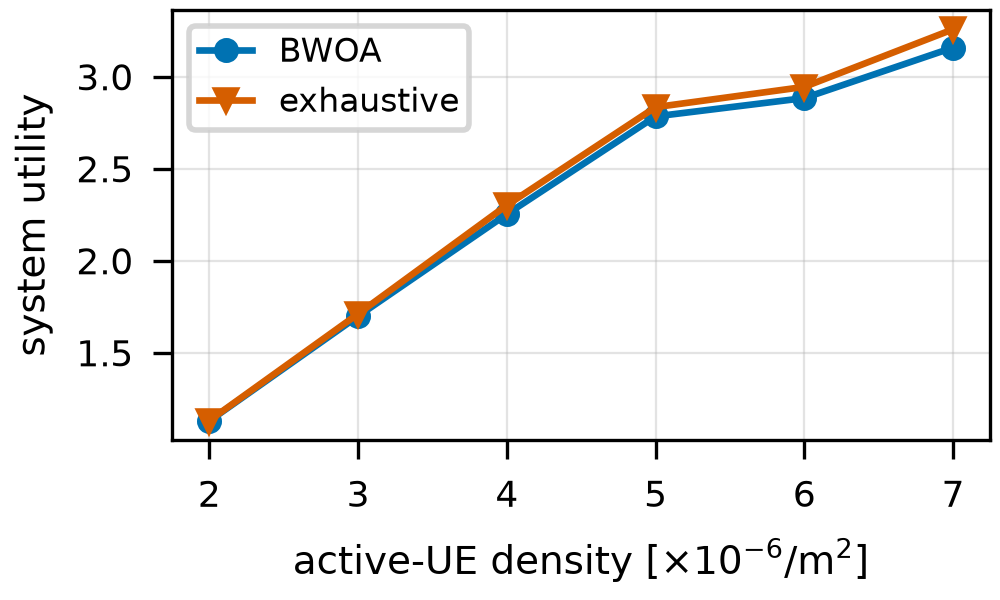
\includegraphics[width=0.49\linewidth]{figures/compare_with_ex_su.png}}
\hfill
\subfloat[]{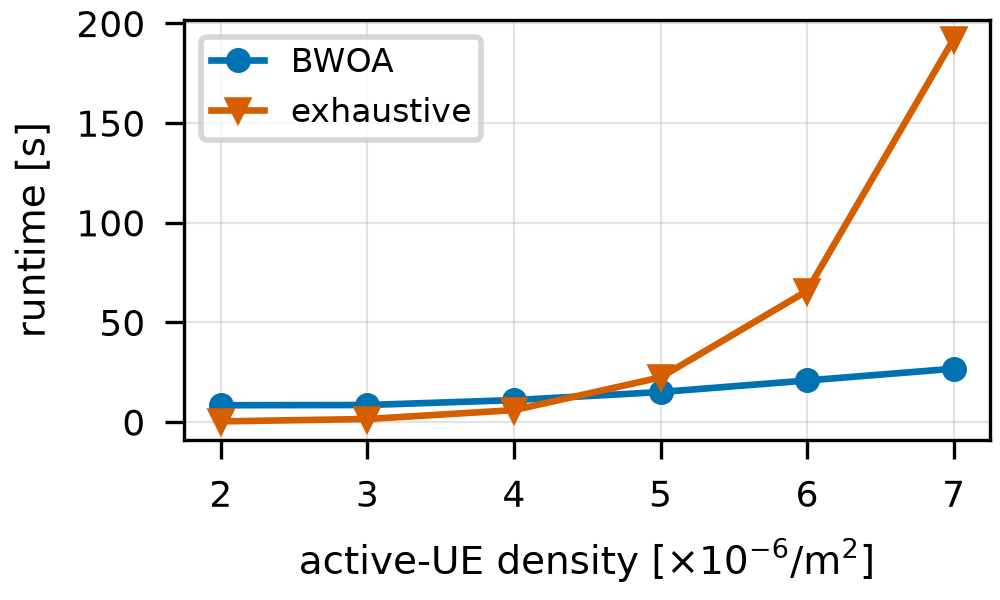
\includegraphics[width=0.49\linewidth]{figures/compare_with_ex_time.png}}
\caption{Proposed BWOA matching versus exhaustive search, $K=3$, $M^{\tt ul}=2$, $M^{\tt dl}=1$: (a) attained utility, (b) runtime, versus active-UE density.}
\label{fig:res}
\end{figure}

Fig.~\ref{fig:res}(a) shows BWOA tracking exhaustive sub-channel search, with a small gap that widens as the association space grows. Fig.~\ref{fig:res}(b) shows the corresponding runtime: exhaustive enumeration is cheaper at low density but grows steeply, whereas BWOA grows near-linearly and overtakes it as density increases. The closed-form ISCC updates leave this curve unchanged.

\begin{figure}[!t]
\centering
\subfloat[]{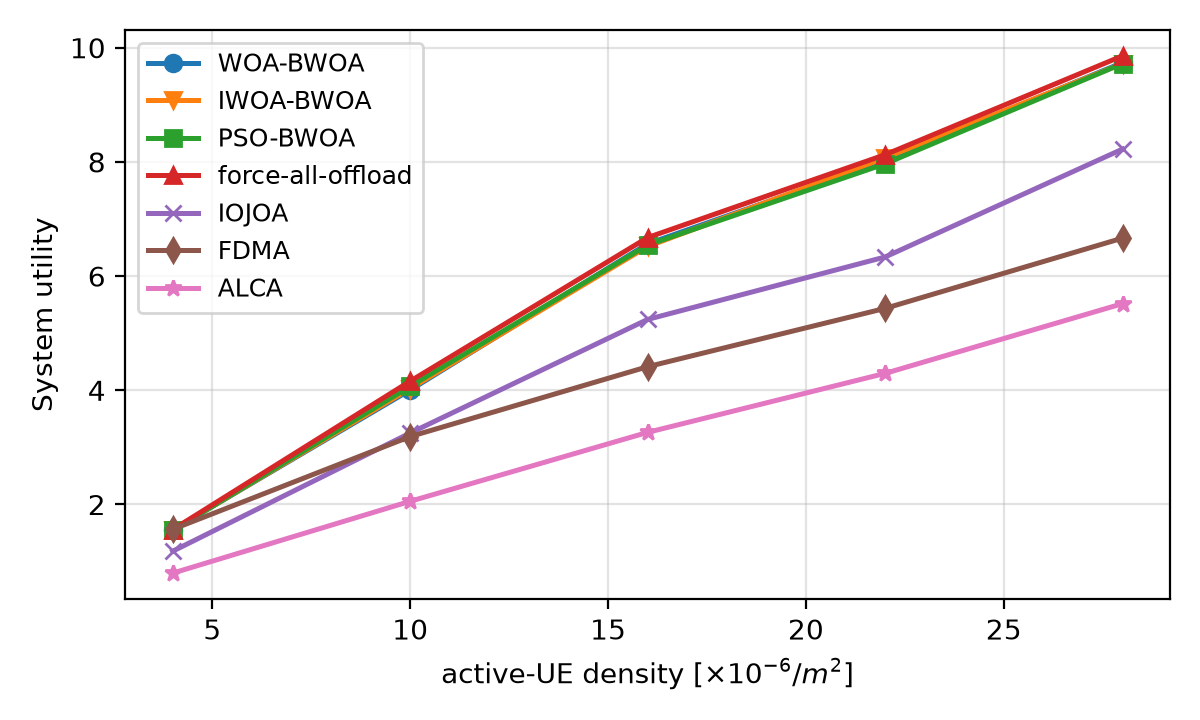
\includegraphics[width=0.49\linewidth]{figures/ue_density_su.png}}
\hfill
\subfloat[]{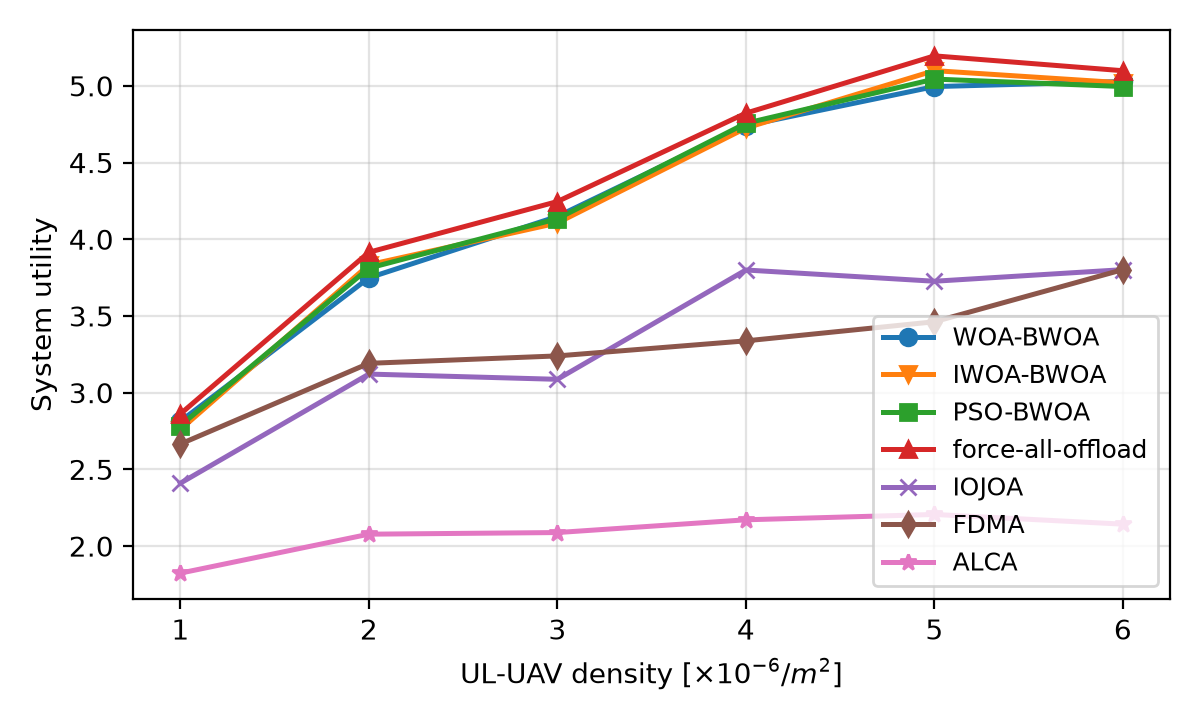
\includegraphics[width=0.49\linewidth]{figures/uav_density_su.png}}
\caption{(a) Utility versus active-UE density for WOA/IWOA/PSO--BWOA (MF-SIC), force-all-offload, IOJOA, FDMA, and ALCA. (b) Utility versus UL UAV-server density.}
\label{fig:res2}
\end{figure}

Fig.~\ref{fig:res2}(a) shows aggregate utility rising with UE density, more terms entering $\mathbb{U}$ even as the co-channel and jamming terms of \eqref{eq:ul_sijnr}--\eqref{eq:dl_sijnr} grow. Fig.~\ref{fig:res2}(b) shows added UAV inference servers changing utility through extra compute and extra G2A/A2G interference.

\begin{figure}[!t]
\centering
\subfloat[]{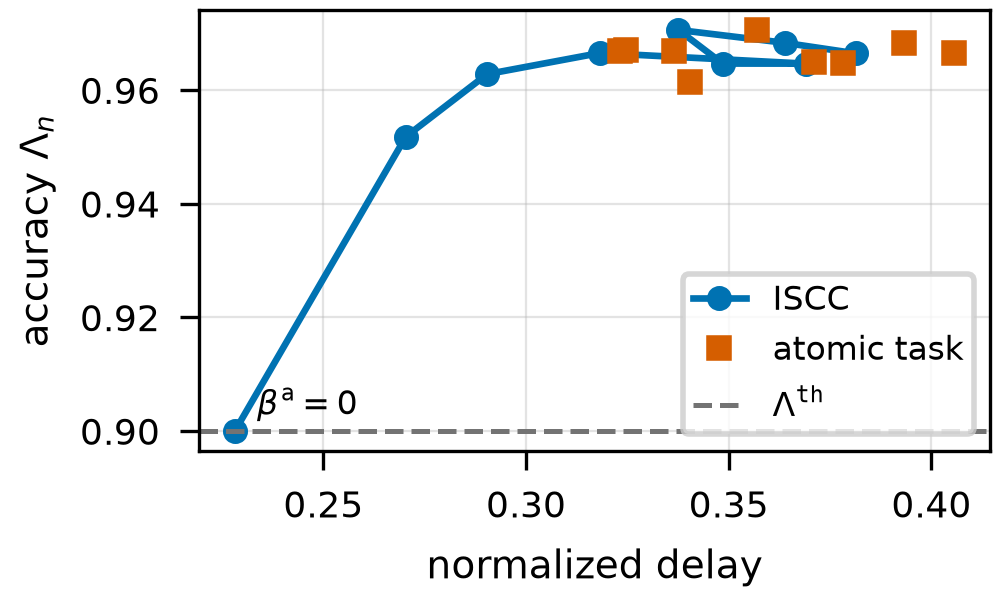
\includegraphics[width=0.49\linewidth]{figures/accuracy_tradeoff.png}}
\hfill
\subfloat[]{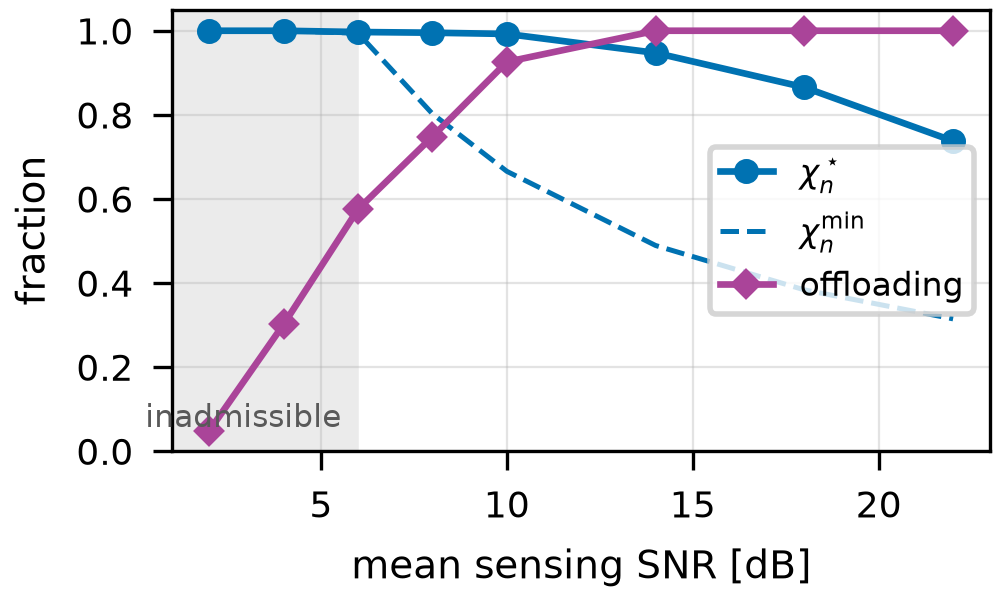
\includegraphics[width=0.49\linewidth]{figures/retention_vs_snr.png}}
\caption{ISCC effects: (a) accuracy--delay frontier swept over $\beta^{\tt a}$, versus the atomic-task baseline; (b) optimal retention $\chi_n^\star$, retention floor $\chi_n^{\min}$, and fraction of offloading UEs versus mean sensing SNR.}
\label{fig:iscc}
\end{figure}

Fig.~\ref{fig:iscc}(a) sweeps $\beta^{\tt a}$ with $\beta^{\tt t}=\beta^{\tt e}=(1-\beta^{\tt a})/2$. At low $\beta^{\tt a}$ retention sits on its floor and accuracy equals $\Lambda^{\tt th}$, with lower delay than the atomic-task point; raising $\beta^{\tt a}$ drives $\chi_n^\star$ to unity, trading latency for accuracy along \eqref{eq:chistar}, until ISCC coincides with the atomic task. In Fig.~\ref{fig:iscc}(b), at low sensing SNR the floor \eqref{eq:chimin} exceeds one, UEs become inadmissible, and offloading collapses; above it, better sensing lowers both $\chi_n^{\min}$ and $\chi_n^\star$: higher-quality observations are compressed \emph{more}, a coupling an atomic-task model cannot express.

\section{Conclusion}
We recast joint UL--DL edge-inference offloading and radio resource management on a SI-TNTN as an ISCC problem combining UAV-mounted servers, planar HPPP geometry with independent altitudes, and jamming-aware MF-SIC/ZFBF SIJNR with sensing-derived tasks, partial offloading, and an inference-accuracy objective. The two sensing-induced variables admit closed forms (a three-point rule for the split and a logarithmic rule for retention), so the MINLP is still solved by the WOA/IWOA/PSO plus BWOA framework at unchanged complexity. Joint sensing-power control and sensing/communication antenna partitioning at the UAV are natural extensions.

\bibliographystyle{IEEEtran}
\bibliography{Bibliography}

\end{document}
